\noindent\textbf{1.}\\
\begin{figure}[H]
  \centering
  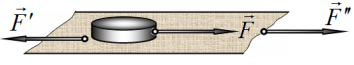
\includegraphics[width=0.35\textwidth]{Figures/Solutions/Fig 1.1.png}
\end{figure}
\noindent Đĩa được tăng tốc bởi lực ma sát $F$ từ băng tải đang chuyển động. Theo định luật III Newton, một lực có độ lớn tương tự $F'$ cũng tác dụng ngược lại lên băng tải. Vì vậy, để băng tải tiếp tục chuyển động với tốc độ không đổi, lực kéo $F''$ phải tăng thêm một lượng đúng bằng lực $F'$ tác động lên băng tải. Công của lực $F$ này cung cấp động năng cho đĩa, đồng thời gây ra sự toả nhiệt.
\begin{figure}[H]
  \centering
  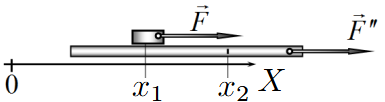
\includegraphics[width=0.35\textwidth]{Figures/Solutions/Fig 1.2.png}
\end{figure}
\noindent Trong hệ quy chiếu gắn với băng tải:
\begin{equation*}
  F = \mu mg \quad \implies \quad a = \frac{F}{m} = \mu g
\end{equation*}
Thời gian để đĩa tăng tốc từ trạng thái tĩnh đến vận tốc $v_0$ của băng tải:
\begin{equation*}
  \tau = \frac{v_0}{a} = \frac{v_0}{\mu g}
\end{equation*}
Trong thời gian này, băng tải đã dịch chuyển đoạn:
\begin{equation*}
  x_2 = v_0 \tau = \frac{v_0^2}{\mu g}
\end{equation*}
Công của lực $F$:
\begin{equation*}
  A = Fx_2 = \mu mg \cdot \frac{v_0^2}{\mu g} = mv_0^2
\end{equation*}
Công này bằng 2 lần động năng mà đĩa nhận được:
\begin{equation*}
  \Delta E = \frac{1}{2}mv_0^2
\end{equation*}
Do đó, lượng nhiệt toả ra là:
\begin{equation*}
  Q = \frac{1}{2}mv_0^2
\end{equation*}
Công của lực ma sát $F$, tác dụng lên đĩa bằng với độ biến thiên động năng của đĩa. Trong khi đó, công của ngoại lực $F''$, có độ lớn bằng $F$, sẽ gấp 2 lần vì trong khoảng thời gian đang xét, băng tải dịch chuyển một đoạn đường gấp đôi.\\

\noindent\textbf{\underline{Cách 2}}: Xét chuyển động của đĩa trong hệ quy chiếu quán tính gắn với băng tải. Trong hệ này, ban đầu đĩa có vận tốc $v_0$, và sau đó dừng lại do ma sát. Do đó, toàn bộ động năng ban đầu của đĩa đã được chuyển hoá thành nhiệt:
\begin{equation*}
  Q = \frac{1}{2}mv_0^2
\end{equation*}

\noindent\textbf{2.} Gọi lực tác dụng lên hạt nhỏ là $F$. Lực này cần được tác dụng để duy trì chuyển động đều của hạt trong chất lỏng. Công của lực này có thể được tính như sau: chia chuyển động của hạt thành nhiều đoạn nhỏ $\Delta x_k$ với lực tác dụng tương ứng trên đoạn thứ $k$ là $F_k$. Khi đó, công của lực là tổng:
\begin{equation*}
  A_1 = \sum_k F_k \Delta x_{1k}
\end{equation*}
Định luật II Newton:
\begin{equation*}
  F_k = m \frac{\Delta v_{1k}}{\Delta t}
\end{equation*}
Với $\Delta v_k$ là độ biến thiên vận tốc của hạt trong khoảng thời gian $\Delta t$. Biến đổi ta được:
\begin{equation*}
  A_1 = \sum_k \left(m \frac{\Delta v_{1k}}{\Delta t}\right) \Delta x_{1k} = \sum_k m \Delta v_{1k} \frac{\Delta x_{1k}}{\Delta t}
  = \sum_k \left(m \frac{\Delta v_{1k}}{\Delta t} \right) \Delta x_{1k}
  = \sum_k m \Delta \left( \frac{v_{1k}^2}{2} \right) = \frac{1}{2}mv_0^2
\end{equation*}
Ta thu được kết quả quen thuộc: công của lực đúng bằng độ biến thiên động năng của hạt. Thực hiện tương tự để tìm công của lực làm chuyển động nước:
\begin{equation*}
  A_2= \sum_{k}F_k \Delta x_{0k}=\sum_{k}m\frac{\Delta v_{1k}}{\Delta t}v_0 \Delta t=\sum_{k}mv_0\Delta v_{1k}=mv_0^2
\end{equation*}
Công của ngoại lực tác dụng lên chất lỏng gấp 2 lần độ biến thiên động năng của hạt, vì vậy phần dư ra chính là nhiệt lượng toả ra do ma sát. Tức nhiệt lượng bằng với động năng thu được của hạt.\\

\begin{wrapfigure}[10]{r}{6cm}
  \centering
  \vspace{-0.55cm}\hspace{-1cm}
  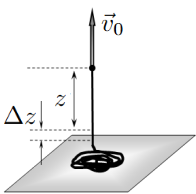
\includegraphics[width=0.28\textwidth]{Figures/Solutions/Fig 1.3.png}
\end{wrapfigure}

\noindent\textbf{3a.} Vì dây xích được nâng lên với vận tốc không đổi nên tại mọi thời điểm, tổng các lực tác dụng lên phần dây đang được nâng bằng 0. Khi dây được nâng lên một đoạn nhỏ $\Delta z$, phần dưới của đoạn này cần được gia tốc nhanh từ 0 đến vận tốc $v_0$. Gia tốc này chỉ có thể có được nhờ lực căng bổ sung trong dây. Lực này có thể được xác định thông qua tốc độ thay đổi xung lượng:
\begin{equation*}
  F' = \frac{\Delta p}{\Delta t} = v_0 \frac{\Delta m}{\Delta t} = v_0 \frac{m}{l} \frac{\Delta z}{\Delta t} = \frac{mv_0^2}{l}
\end{equation*}
Trong đó $\Delta m = \dfrac{m}{l} \Delta z = \dfrac{m}{l}v_0 \Delta t$ là khối lượng của phần dây được nâng lên khỏi bàn trong khoảng thời gian ngắn $\Delta t$. Khi đó, lực kéo dây lên với vận tốc không đổi sẽ bằng tổng của trọng lực tác dụng lên phần dây đã được nâng $m'g = \dfrac{m}{l} z g$ và lực $F'$ đã tính ở trên:
\begin{equation*}
  F = \frac{m}{l} z g + \frac{m}{l} v_0^2
\end{equation*}

\noindent\textbf{3b.}
\begin{figure}[H]
  \centering
  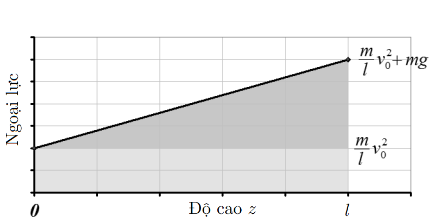
\includegraphics[width=0.6\textwidth]{Figures/Solutions/Fig 1.4.png}
\end{figure}

\noindent Công của lực vừa tìm được bằng diện tích bên dưới đồ thị biểu diễn sự phụ thuộc của lực theo độ dịch chuyển:
\begin{equation*}
  A = \left(\frac{mv_0^2}{l}\right) l + \frac{1}{2}mgl = mv_0^2 + \frac{1}{2}mgl
\end{equation*}
Năng lượng cung cấp cho dây xích dùng để tăng động năng của dây lên một lượng $\frac{1}{2}mv_0^2$, tăng thế năng lên một lượng $\frac{1}{2}mgl$, và một phần chuyển thành nhiệt năng $Q$. Do đó:
\begin{equation*}
  A = mv_0^2 + \frac{1}{2}mgl = \frac{1}{2}mv_0^2 + \frac{1}{2}mgl + Q
\end{equation*}
Do đó, nhiệt lượng toả ra là:
\begin{equation*}
  Q = \frac{1}{2}mv_0^2
\end{equation*}




